
\documentclass[11pt,letterpaper]{article}

% Load some basic packages that are useful to have
% and that should be part of any LaTeX installation.
%
% be able to include figures
\usepackage{graphicx}
% get nice colors
\usepackage{xcolor}

% change default font to Palatino (looks nicer!)
\usepackage[latin1]{inputenc}
\usepackage{mathpazo}
\usepackage[T1]{fontenc}
% load some useful math symbols/fonts
\usepackage{latexsym,amsfonts,amsmath,amssymb}

% comfort package to easily set margins
\usepackage[top=1in, bottom=1in, left=1in, right=1in]{geometry}

% control some spacings
%
% spacing after a paragraph
\setlength{\parskip}{.15cm}
% indentation at the top of a new paragraph
\setlength{\parindent}{0.0cm}


\begin{document}

\begin{center}
\Large
Ay190 -- Worksheet 10\\
Anthony Alvarez\\
Date: February 18, 2014
\end{center}

\section{Advection Equation}

We will consider the advection equation.
$$ \frac{\partial u}{\partial t} + v \frac{\partial u}{\partial x} = 0$$

We use it to advect a Gaussian $$ \Psi_0 = \Psi(x,t=0) = e^{-(x-x_0)^2/(2\sigma^2))}$$.
Where $x_0 = 30$ and $\sigma^2 = 15$. We initially choose a positive velocity
$v=0.1$ in a $[0,100]$ domain. 

\subsection{Moving Analytic Gaussian}

As you can see in myadvect.py I have implemented the moving analytic Gaussian.

What I notice happening is it slowly moves to the right as it updates. Since, 
it is the anlaytic version it does not change shape or height as no errors
accumulate. 

\subsection{Upwind Advection}

When we implement the upwind advection we notice that it is stable for 
$0\leq \alpha = \frac{v\delta t}{\delta x}$. Se can see in ~\ref{fig:upwind1}
and in ~\ref{fig:upwind2} that the upwind scheme (Shown in blue) flattens and
spreads out over time. This contribues to the error which can be seen in
~\ref{fig:upwinderr}. We can see that although this system accumulates error it 
is still in some sense stable. 

\begin{figure}[bth]
\centering
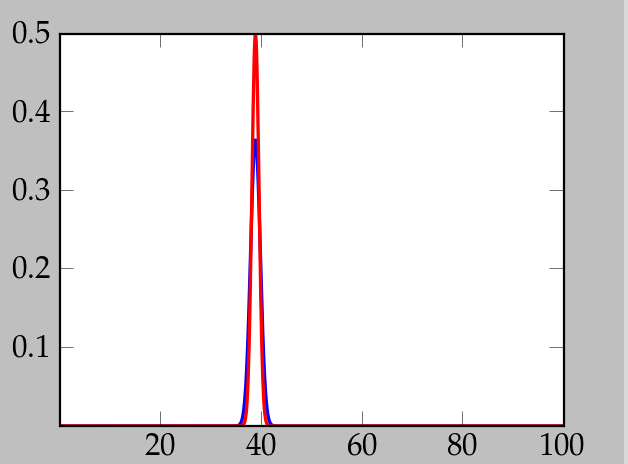
\includegraphics[width=0.5\textwidth]{Upwind1.png}
\caption{Upwind scheme after a small amount of time. Upwind in Blue, Analytic in Red.}
\label{fig:upwind1}
\end{figure}

\begin{figure}[bth]
\centering
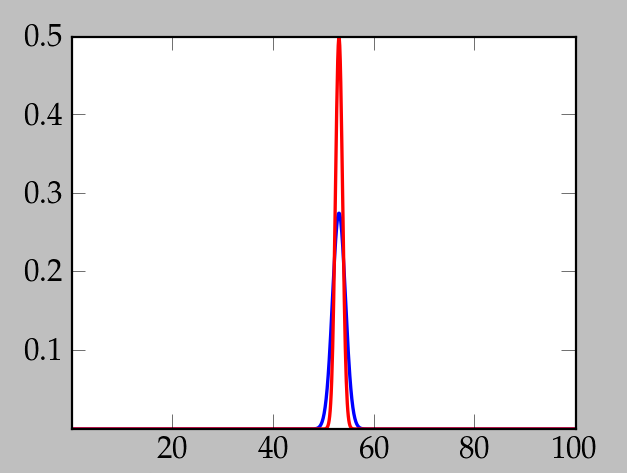
\includegraphics[width=0.5\textwidth]{Upwind2.png}
\caption{Upwind scheme after a longer time. Upwind in Blue, Analytic in Red.}
\label{fig:upwind2}
\end{figure}

\begin{figure}[bth]
\centering
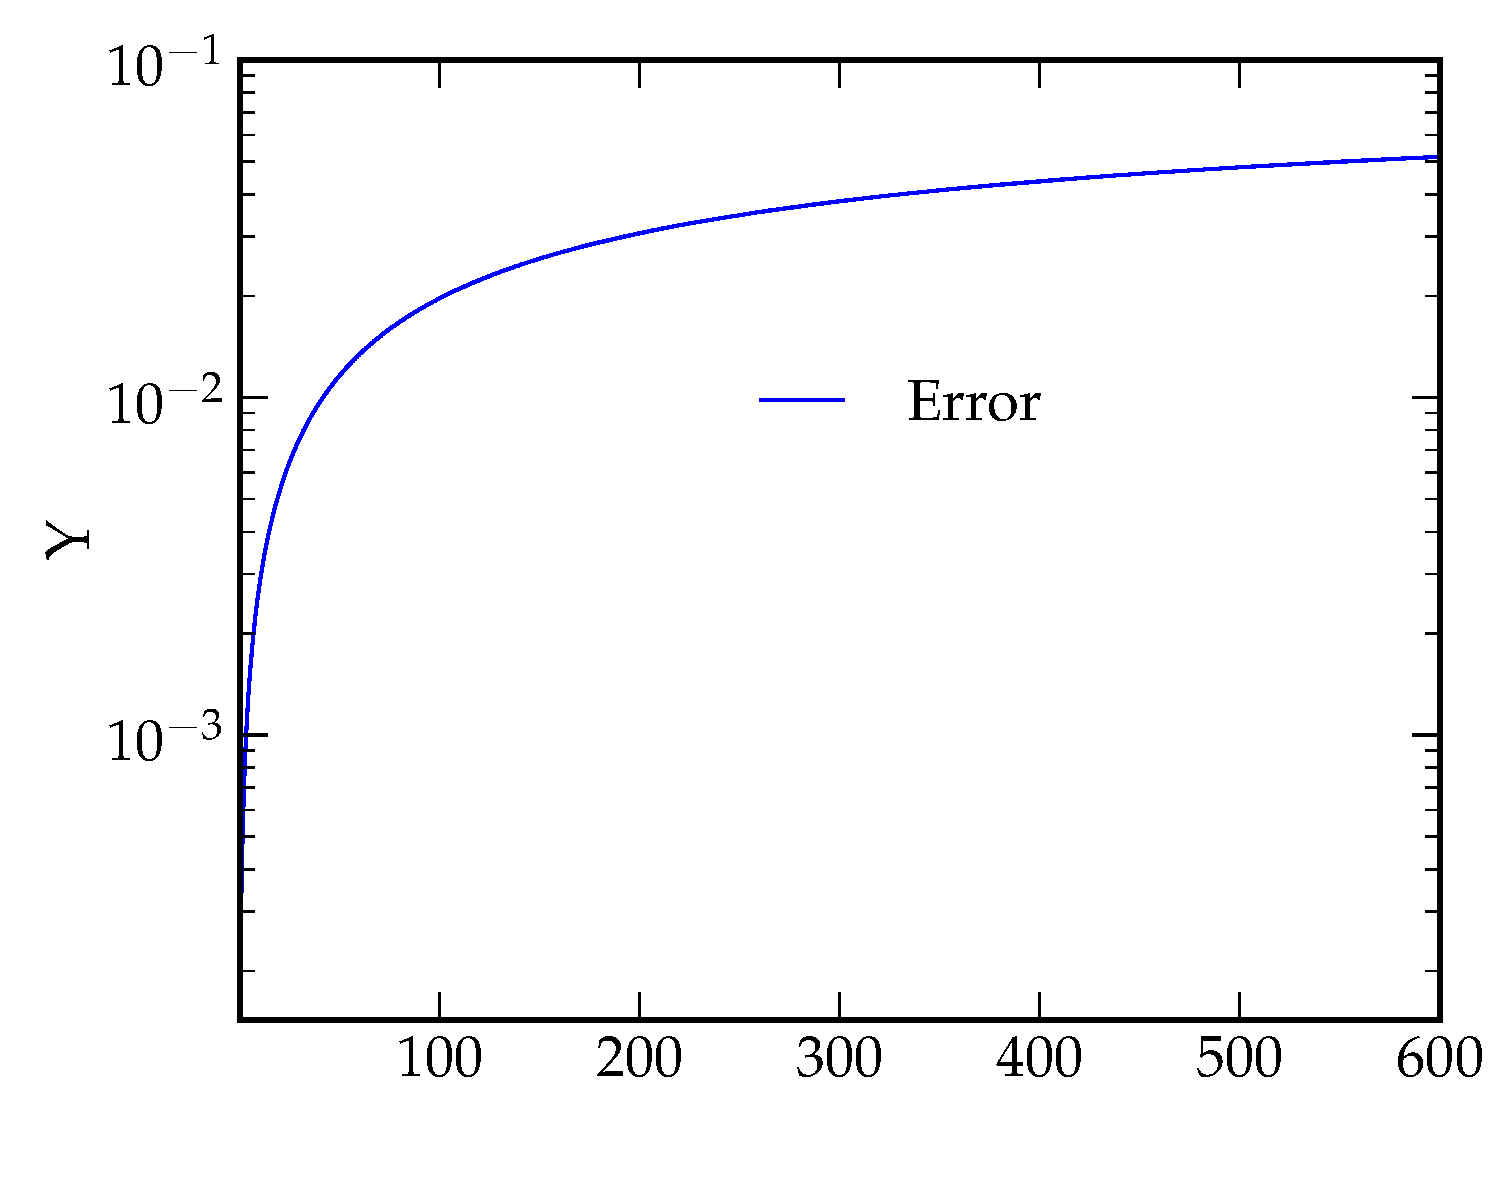
\includegraphics[width=0.5\textwidth]{2.pdf}
\caption{Error in upwind scheme for $\alpha < 1$ over time.}
\label{fig:upwinderr}
\end{figure}

When we implement the same upwind scheme with $\alpha > 1$ we can see that this 
system is highly unstable, the error is completely unbounded and grows out of
control as we can see in ~\ref{fig:upwindBIGerr}

\begin{figure}[bth]
\centering
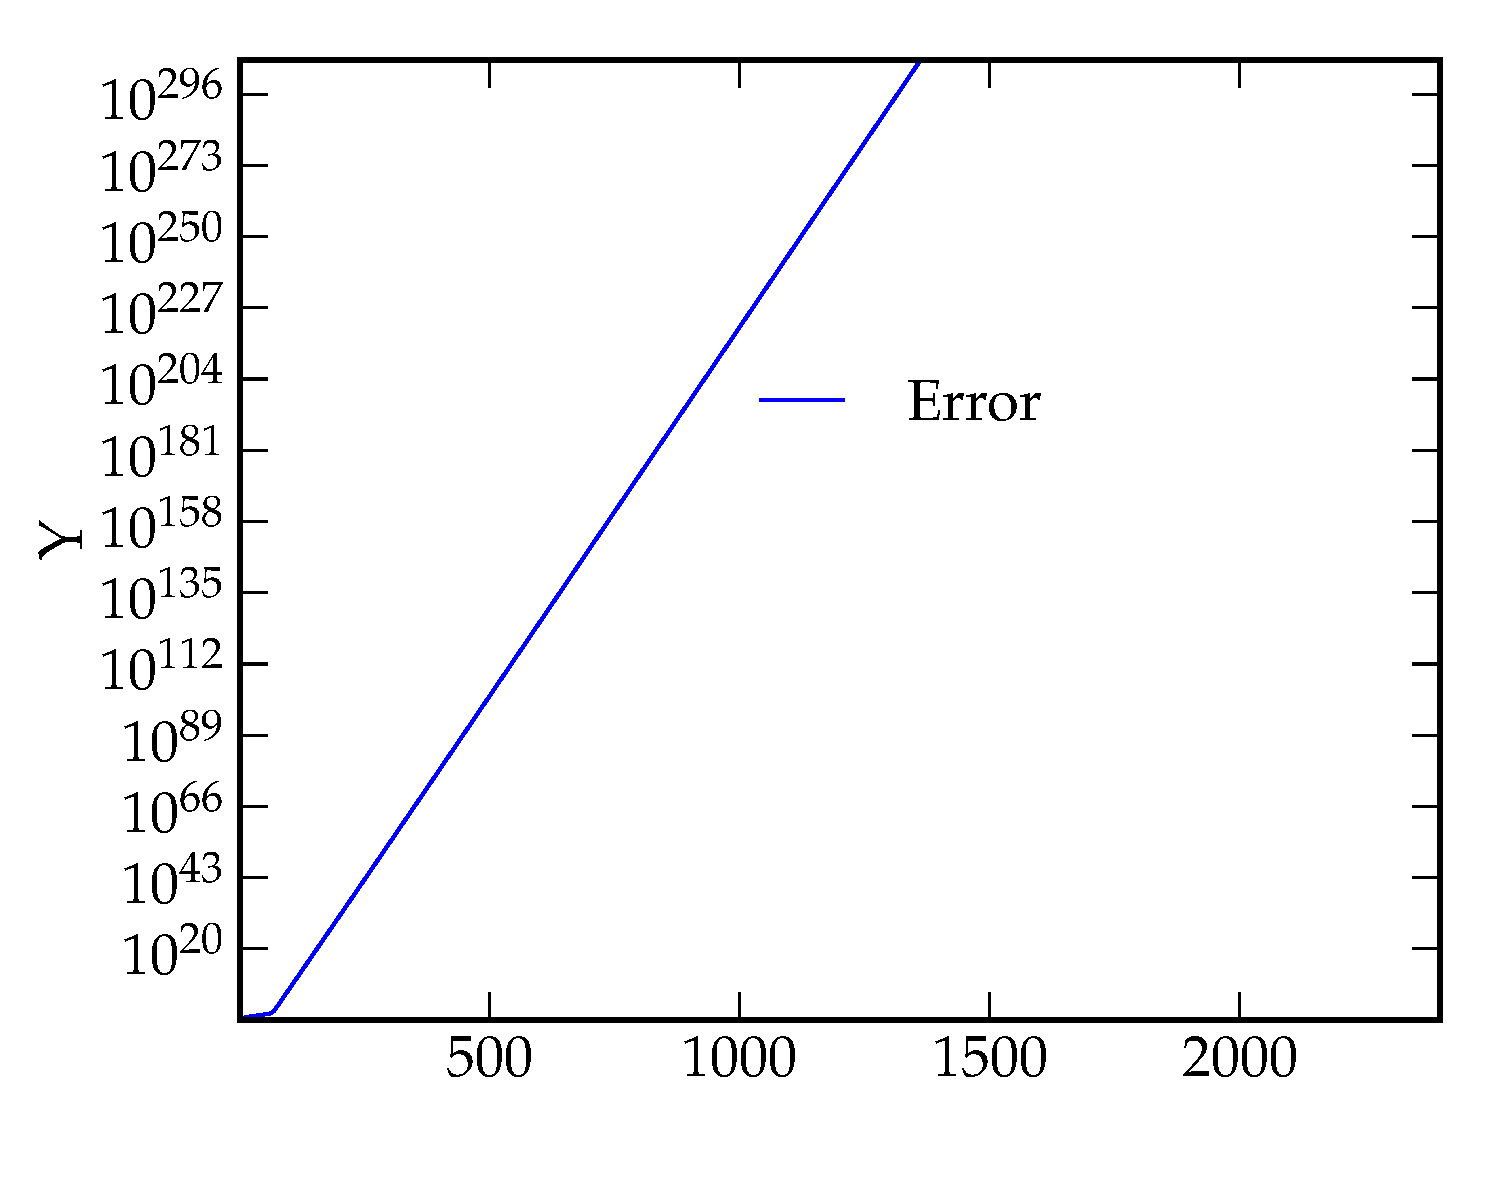
\includegraphics[width=0.5\textwidth]{2b.pdf}
\caption{Error in upwind scheme for $\alpha > 1$. The error seems totally unbounded. }
\label{fig:upwindBIGerr}
\end{figure}

When we try a Gaussian with a $\sigma$ five times smaller we find that the 
upwind scheme performs equivalently visually, no plots shown. But that it does
accumulate errors more wuickly as we can see in ~\ref{fig:upwindSmallSigma}.
This is probably due to the increased sharpness of the curve. 

\begin{figure}[bth]
\centering
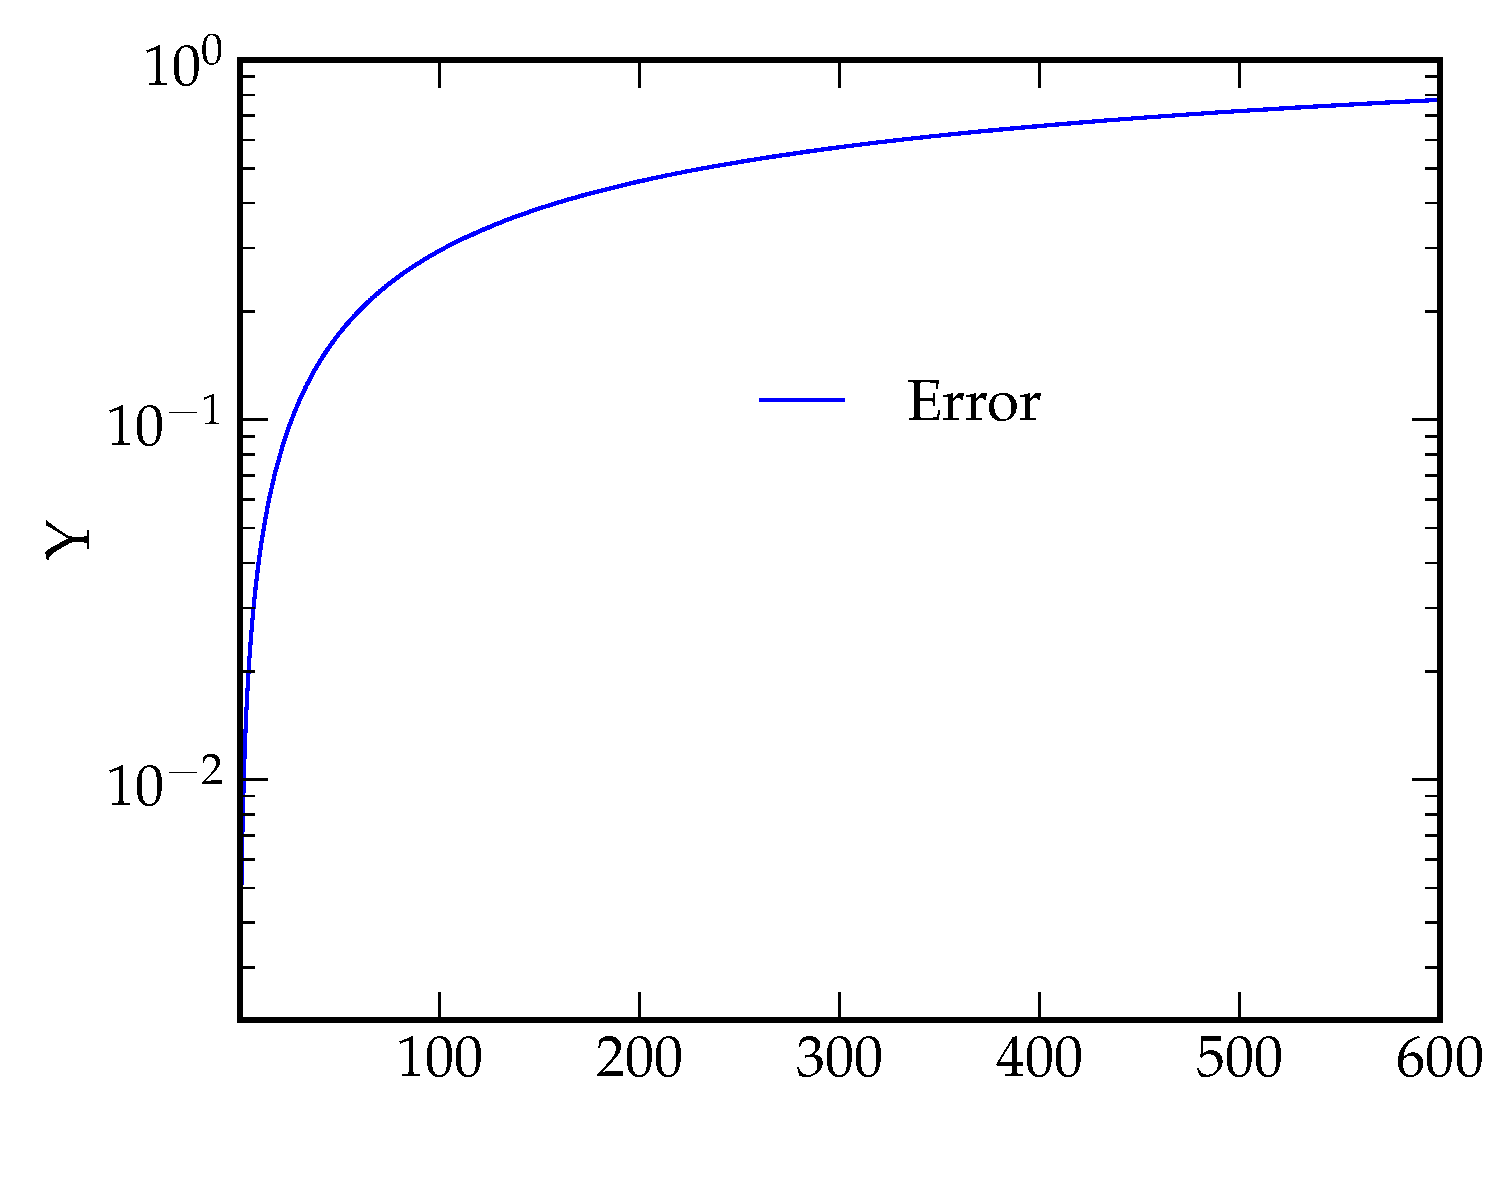
\includegraphics[width=0.5\textwidth]{2c.pdf}
\caption{Error in upwind scheme for $\alpha < 1, \sigma = \frac{\sqrt{15}}{5}$ }
\label{fig:upwindSmallSigma}
\end{figure}

\subsection{FTCS}

Se can see in ~\ref{fig:upwind3} that a small instability quickly develops.
Later the instability grows and spawns a smaller
instability further left of the true peak as we can see in ~\ref{fig:upwind4}. 
Eventually the left most instability grows to eclipse everything as we can see 
in ~\ref{fig:upwind5}. These massive instabilites contribue to the error which
 can be seen in ~\ref{fig:upwindBIGerr}. We can see that this system accumulates
a massive amount of error and is in no sense stable.

\begin{figure}[bth]
\centering
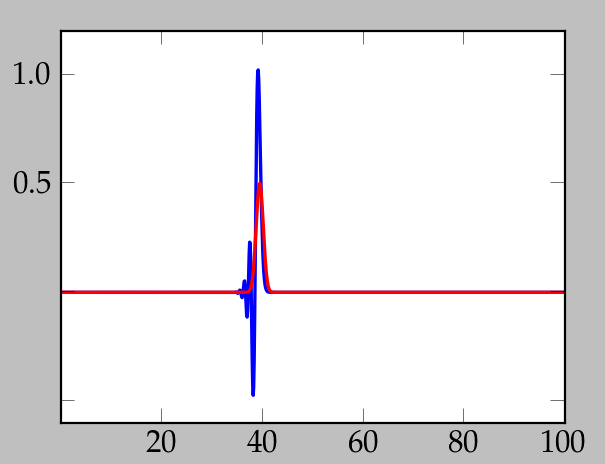
\includegraphics[width=0.5\textwidth]{Upwind3.png}
\caption{FTCS scheme after a small amount of time. Notice thes small instability. FTCS in Blue, Analytic in Red.}
\label{fig:upwind3}
\end{figure}

\begin{figure}[bth]
\centering
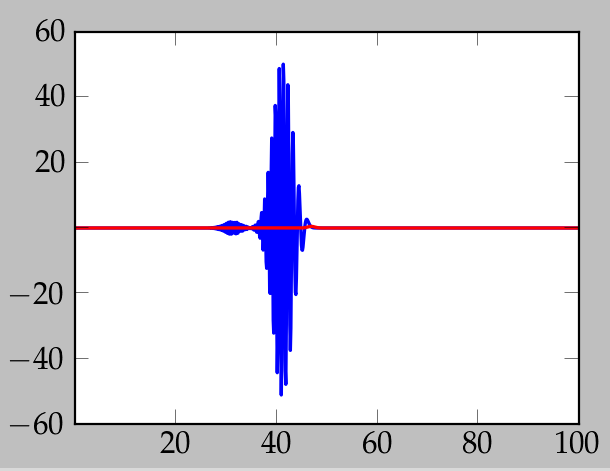
\includegraphics[width=0.5\textwidth]{Upwind4.png}
\caption{FTCS scheme after a longer time. The instability grows significantly. FTCS in Blue, Analytic in Red.}
\label{fig:upwind4}
\end{figure}

\begin{figure}[bth]
\centering
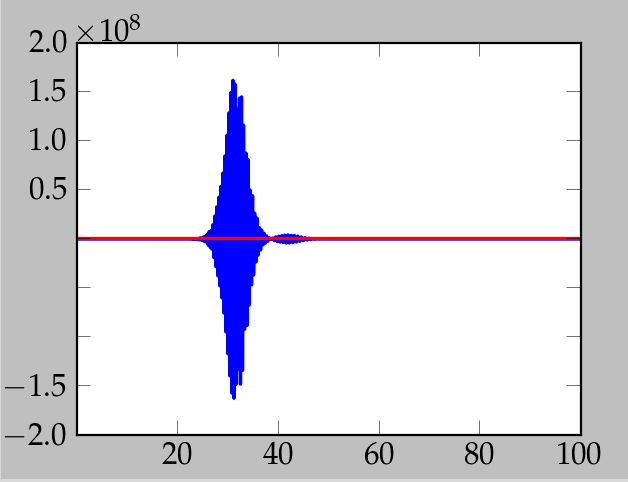
\includegraphics[width=0.5\textwidth]{Upwind5.png}
\caption{FTCS scheme after a longer time. The instability now dominates completely. FTCS in Blue, Analytic in Red.}
\label{fig:upwind5}
\end{figure}

\subsection{Lax-Friedrich Method}

We implement the Lax-Friedrich method and as we can see in ~\ref{fig:LFM1} and 
~\ref{fig:LFM2}. The Lax-Friedrich method has a similar flattening process as 
the upwind method seen in ~\ref{fig:upwind1} and ~\ref{fig:upwind2}. At least 
visually these methods produce very similar results. 

\begin{figure}[bth]
\centering
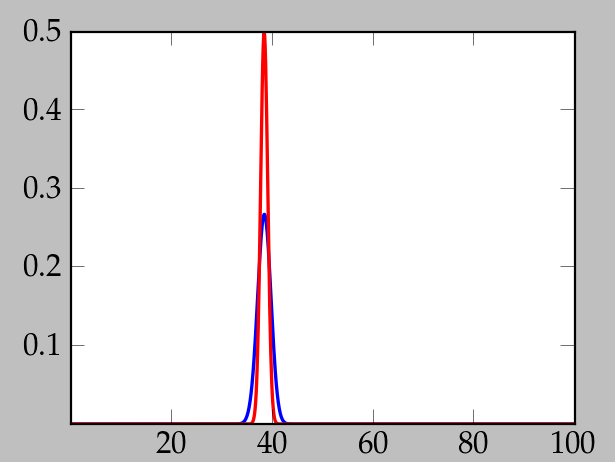
\includegraphics[width=0.5\textwidth]{LFM1.png}
\caption{Lax-Friedrich method scheme after a short time. The numerical result flattens out slightly. Lax-Friedrich method in Blue, Analytic in Red.}
\label{fig:LFM1}
\end{figure}


\begin{figure}[bth]
\centering
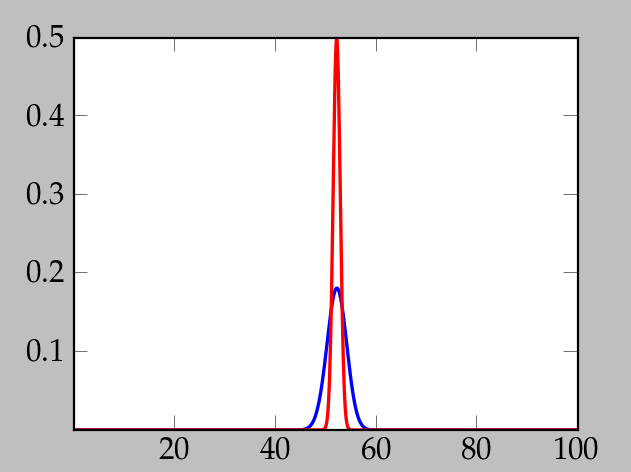
\includegraphics[width=0.5\textwidth]{LFM2.png}
\caption{Lax-Friedrich method scheme after a longer time. The numerical result flattens out slightly. Lax-Friedrich method in Blue, Analytic in Red.}
\label{fig:LFM2}
\end{figure}


\end{document}




